% Provenance (never printed): cycle 3 "La planete Terre" (natural phenomena
% and the risks they bring: storms, floods, droughts, earthquakes, eruptions;
% warnings and the right behaviour); see sources/book1/PROVENANCE.md.
% Book 1, grade 5, chapter 3.
\chapter{Les aléas naturels}\label{ch:g5:natural-hazards}

C'est vendredi soir. À la radio, la musique s'arrête et une voix calme lit
une alerte~: une forte \omterm{def:g5:natural-hazards:storm}{tempête} atteindra la \omterm{def:g1:landscapes-around-us:water}{côte} cette nuit, avec des vents
très violents et de fortes \omterm{def:g4:clouds-rain-snow:precipitation}{pluies}. On demande à chacun de rester à
l'intérieur à partir de neuf heures, et d'attacher ou de rentrer tout ce
que le vent pourrait emporter.

La famille de Lena se met au travail. Son père range les chaises et la
table du jardin dans la cabane. Sa mère vérifie que les lampes de poche
fonctionnent et pose des piles de rechange sur la table de la cuisine. Lena
remplit d'eau deux grandes bouteilles. À neuf heures, tout le monde est à
l'intérieur, et le vent hurle déjà.

\begin{omfigure}
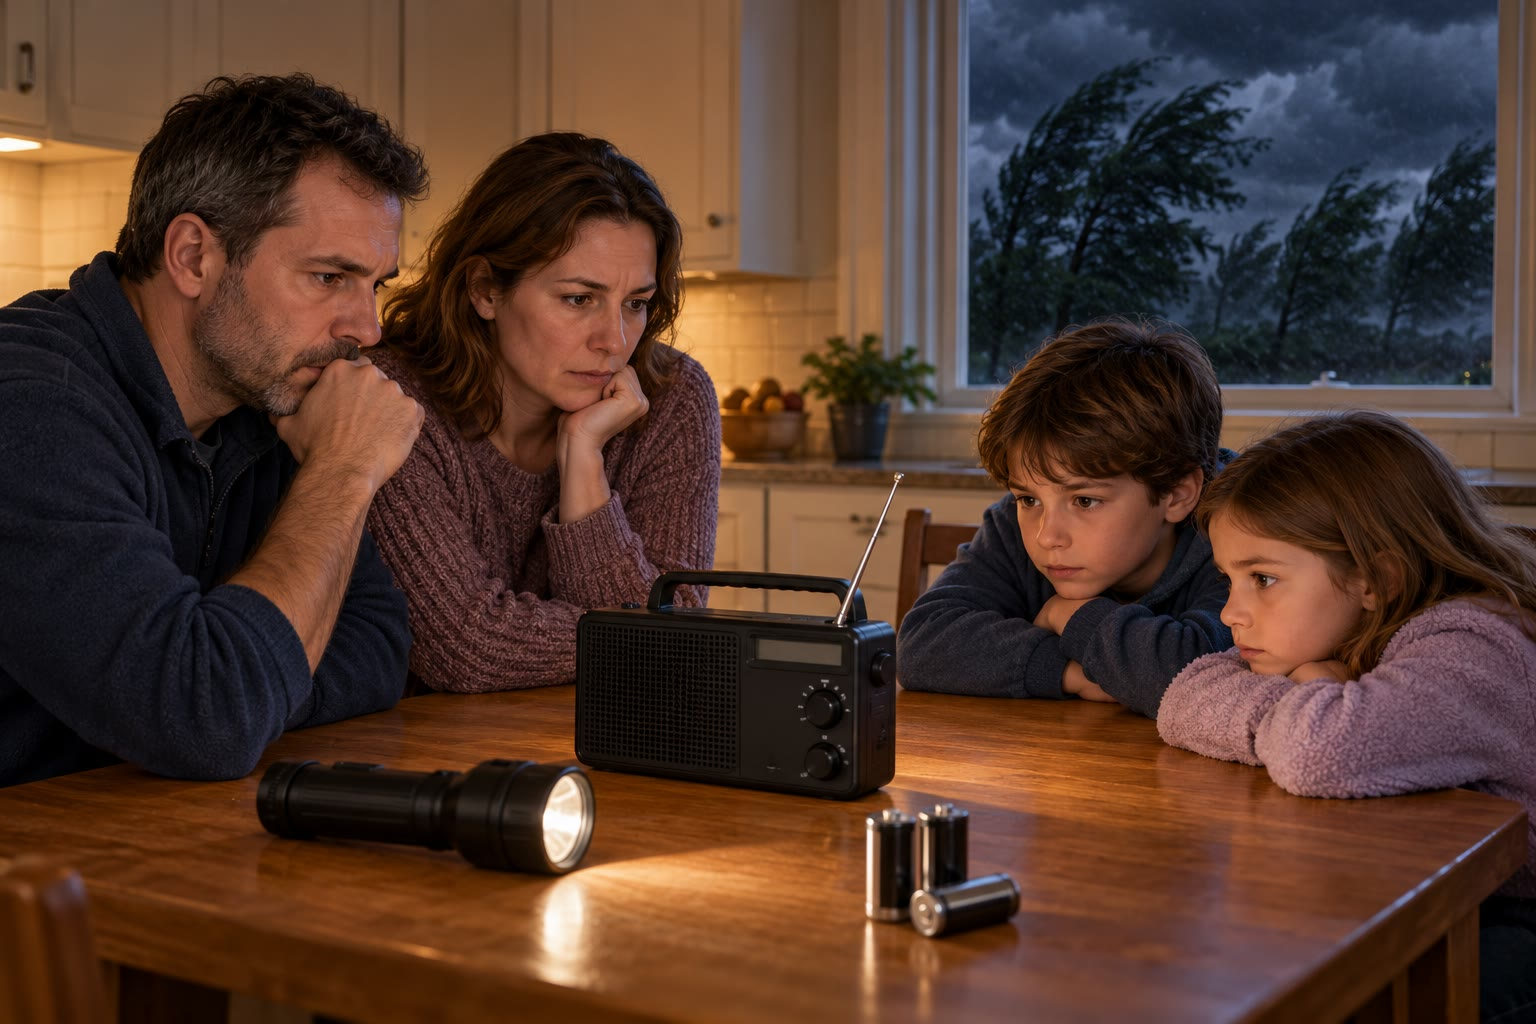
\includegraphics[width=0.5\linewidth]{images/book1/ai/g5-radio-warning.jpg}

{\small Une famille écoute une alerte à la \omterm{def:g5:natural-hazards:storm}{tempête} à la radio, avec les
lampes de poche et les piles de rechange prêtes.}
\end{omfigure}

\begin{recall}
Un \omterm{def:g4:volcanoes-earthquakes-first-look:volcano}{volcan} peut entrer en \omterm{def:g4:volcanoes-earthquakes-first-look:eruption}{éruption} et projeter de la \omterm{def:g4:volcanoes-earthquakes-first-look:eruption}{lave}, des cendres et
des gaz~; un \omterm{def:g4:volcanoes-earthquakes-first-look:earthquake}{séisme} est une secousse soudaine du sol~; pendant un \omterm{def:g4:volcanoes-earthquakes-first-look:earthquake}{séisme},
on se baisse, on s'abrite et on s'agrippe
(\cref{ch:g4:volcanoes-earthquakes-first-look}). Une \omterm{def:g1:landscapes-around-us:water}{rivière} qui reçoit
plus d'eau que son lit ne peut en contenir inonde sa \omterm{def:g5:water-shapes-the-land:flood}{plaine d'inondation}
(\cref{ch:g5:water-shapes-the-land}). Chaque lieu a son propre \omterm{def:g5:weather-and-climate:climate}{climat}, et
les zones chaude, tempérées et froides font le tour du \omterm{def:g3:continents-and-oceans:globe}{globe}
(\cref{ch:g5:weather-and-climate}).
\end{recall}

\section{Qu'est-ce qu'un aléa naturel~?}

La nature n'est pas toujours calme. Le vent peut souffler assez fort pour
casser des arbres, les \omterm{def:g1:landscapes-around-us:water}{rivières} peuvent déborder, le sol peut trembler. Ces
événements font partie du fonctionnement de la Terre~: ils se produisaient
bien avant qu'il y ait des hommes, et ils continueront de se produire.

\begin{definition}[Aléa naturel]\label{def:g5:natural-hazards:hazard}
Un \emph{aléa naturel}\index{alea naturel@aléa naturel} est un phénomène
naturel qui peut blesser des personnes ou endommager ce qu'elles ont
construit~: une \omterm{def:g5:natural-hazards:storm}{tempête}, une inondation, une \omterm{def:g5:natural-hazards:drought}{sécheresse}, un \omterm{def:g4:volcanoes-earthquakes-first-look:earthquake}{séisme}, une
\omterm{def:g4:volcanoes-earthquakes-first-look:eruption}{éruption} volcanique, un \omterm{def:g5:natural-hazards:landslide}{glissement de terrain}{\ldots}
\end{definition}

Nous pouvons classer les \omterm{def:g5:natural-hazards:hazard}{aléas naturels} selon leur origine~: l'air, l'eau
ou le sol.

\begin{omfigure}
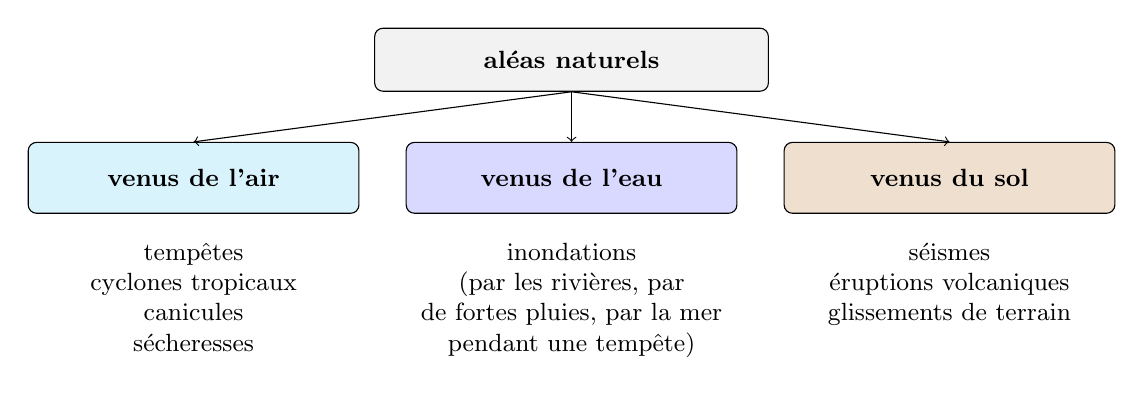
\begin{tikzpicture}[font=\small, box/.style={draw, rounded corners=3pt,
    minimum width=4.2cm, minimum height=0.9cm, align=center}]
  \node[box, fill=cyan!15, font=\small\bfseries] (A) at (0,0) {venus de l'air};
  \node[box, fill=blue!15, font=\small\bfseries] (W) at (4.8,0) {venus de l'eau};
  \node[box, fill=brown!25, font=\small\bfseries] (G) at (9.6,0) {venus du sol};
  \node[align=center, anchor=north] at (0,-0.7) {tempêtes\\cyclones tropicaux\\canicules\\sécheresses};
  \node[align=center, anchor=north] at (4.8,-0.7) {inondations\\(par les rivières, par\\de fortes pluies, par la mer\\pendant une tempête)};
  \node[align=center, anchor=north] at (9.6,-0.7) {séismes\\éruptions volcaniques\\glissements de terrain};
  \node[draw, rounded corners=3pt, fill=gray!10, font=\small\bfseries,
    minimum width=5cm, minimum height=0.8cm] (N) at (4.8,1.5) {aléas naturels};
  \draw[->] (N.south) -- (A.north);
  \draw[->] (N.south) -- (W.north);
  \draw[->] (N.south) -- (G.north);
\end{tikzpicture}

{\small Les \omterm{def:g5:natural-hazards:hazard}{aléas naturels}, classés selon leur origine.}
\end{omfigure}

\section{Les aléas venus de l'air}

\begin{definition}[Tempête]\label{def:g5:natural-hazards:storm}
Une \emph{tempête}\index{tempete@tempête} est une période de vent très
fort, généralement accompagnée de fortes \omterm{def:g4:clouds-rain-snow:precipitation}{pluies} ou de \omterm{def:g4:clouds-rain-snow:precipitation}{neige}, et parfois
d'orage, avec du tonnerre et des éclairs.
\end{definition}

Une forte \omterm{def:g5:natural-hazards:storm}{tempête} casse des branches, abat des arbres, arrache les tuiles
des toits et peut projeter des chaises de jardin à travers les fenêtres.
Sur la \omterm{def:g1:landscapes-around-us:water}{côte}, son vent pousse la \omterm{def:g2:water-on-earth:ocean}{mer} contre le rivage et envoie d'énormes
vagues par-dessus les digues.

Les \omterm{def:g5:natural-hazards:storm}{tempêtes} les plus puissantes de la Terre se forment au-dessus des \omterm{def:g2:water-on-earth:ocean}{mers}
tropicales chaudes. Ce sont d'immenses \omterm{def:g5:natural-hazards:storm}{tempêtes} qui tournent sur
elles-mêmes~: vues de l'espace, elles ressemblent à une gigantesque spirale
de \omterm{def:g4:clouds-rain-snow:cloud}{nuages}, avec au milieu un trou calme et dégagé, l'œil. Autour de l'œil
soufflent les vents les plus forts. Ce même genre de \omterm{def:g5:natural-hazards:storm}{tempête} porte des noms
différents selon les \omterm{def:g2:water-on-earth:ocean}{océans}~: on l'appelle \emph{ouragan} dans
l'Atlantique Nord et dans le Pacifique Est, \emph{typhon} dans le
Pacifique Nord-Ouest, et \emph{cyclone tropical} dans le Pacifique Sud et
dans l'\omterm{def:g2:water-on-earth:ocean}{océan} Indien.
% ledger: noaa:cyclone-names

\begin{omfigure}
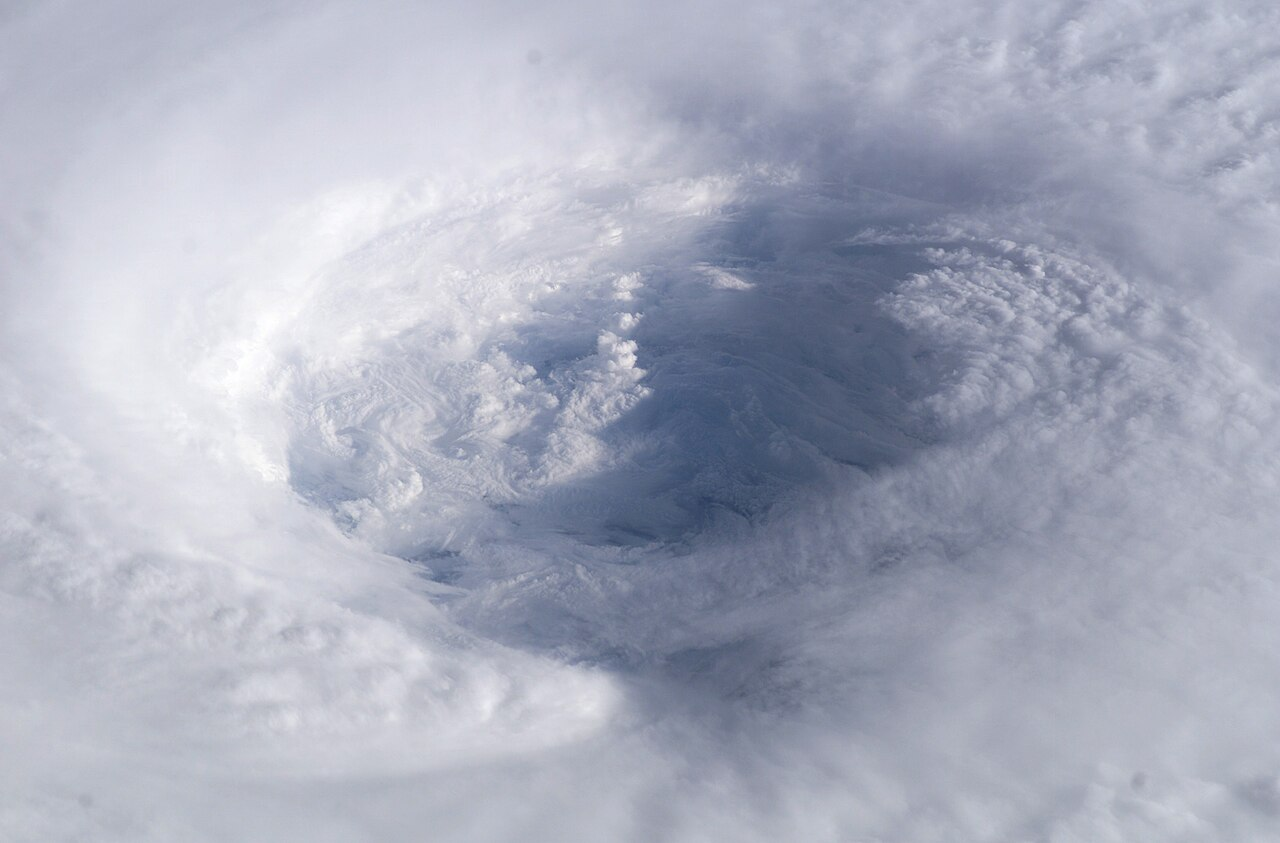
\includegraphics[width=0.5\linewidth]{images/book1/g5-hurricane-isabel-iss.jpg}

{\small Vue plongeante dans l'œil de l'ouragan Isabel, au-dessus de l'\omterm{def:g2:water-on-earth:ocean}{océan}
Atlantique, en septembre 2003, depuis la Station spatiale internationale~:
une muraille de \omterm{def:g4:clouds-rain-snow:cloud}{nuages} autour d'un centre plus calme. Photographie~: NASA
(domaine public).}
% ledger: nasa:isabel-iss
\end{omfigure}

Certains aléas venus de l'air sont lents et silencieux. Une
\emph{canicule} est une période de plusieurs jours et plusieurs nuits
beaucoup plus chauds que d'habitude. Elle est dangereuse surtout pour les
personnes très âgées, les bébés et les malades.

\begin{definition}[Sécheresse]\label{def:g5:natural-hazards:drought}
Une \emph{sécheresse}\index{secheresse@sécheresse} est une longue période,
de plusieurs mois ou même de plusieurs années, avec beaucoup moins de \omterm{def:g4:clouds-rain-snow:precipitation}{pluie}
que d'habitude en ce lieu. Le sol se dessèche, les \omterm{def:g1:landscapes-around-us:water}{rivières} et les \omterm{def:g1:landscapes-around-us:water}{lacs}
rétrécissent, les cultures se fanent et meurent.
\end{definition}

Une \omterm{def:g5:natural-hazards:drought}{sécheresse} s'installe lentement~: personne ne peut dire quel jour elle
commence. Mais une longue \omterm{def:g5:natural-hazards:drought}{sécheresse} peut laisser les agriculteurs sans
récolte et les villes à court d'eau.

\begin{omfigure}
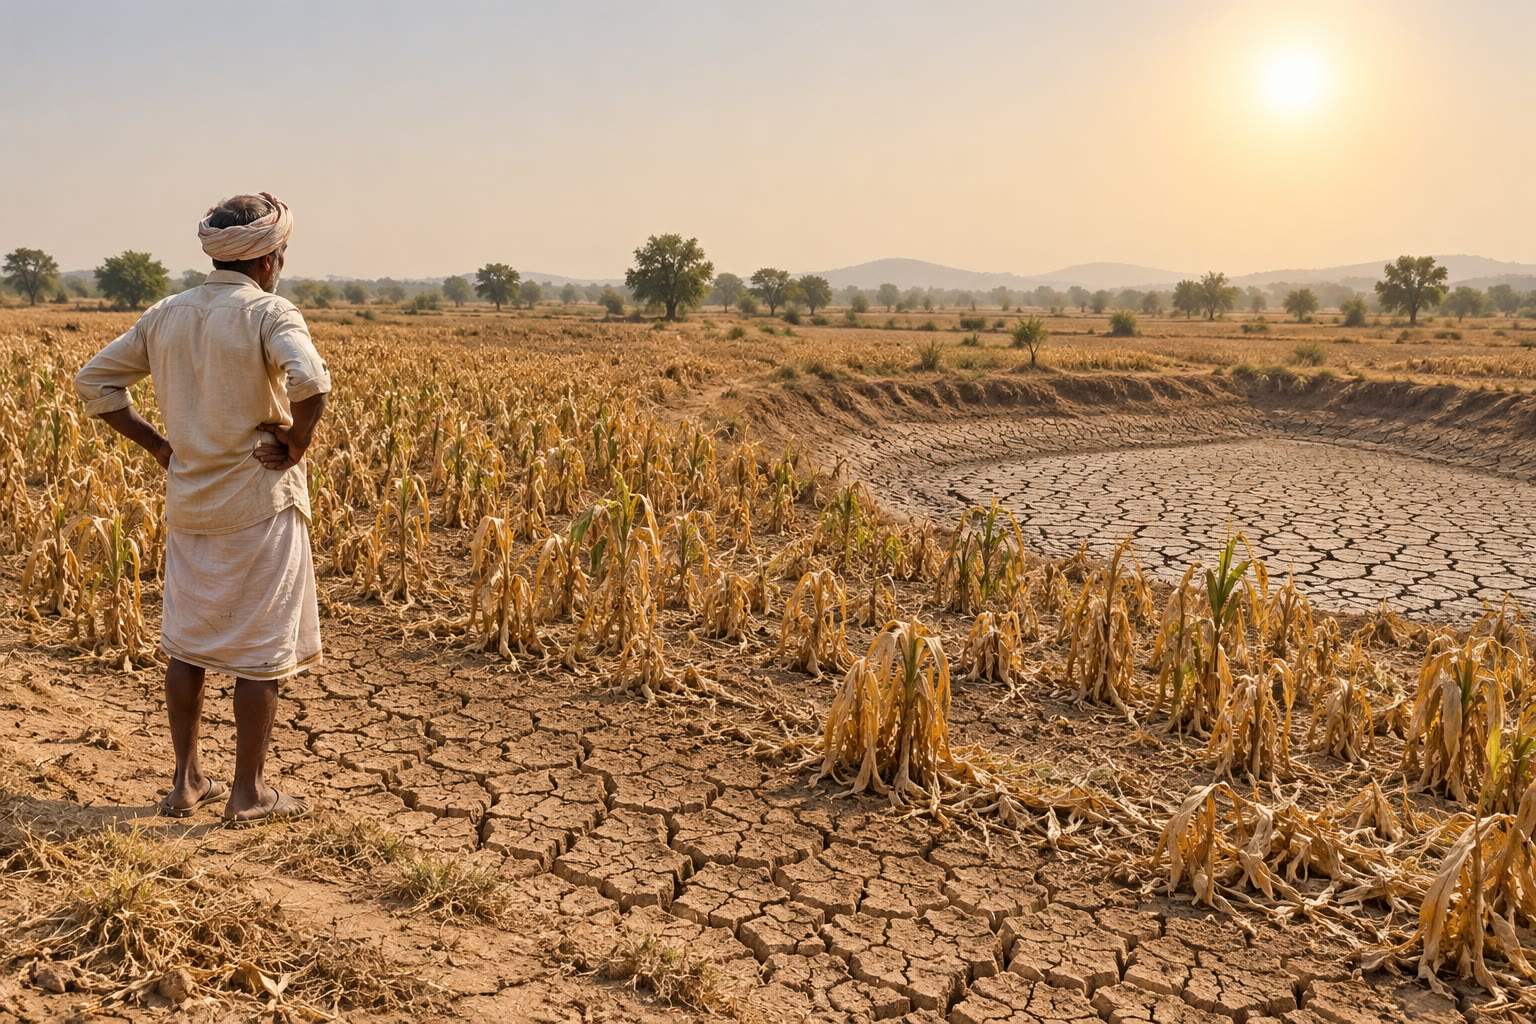
\includegraphics[width=0.42\linewidth]{images/book1/ai/g5-drought-field.jpg}

{\small Un champ pendant une longue \omterm{def:g5:natural-hazards:drought}{sécheresse}~: la terre est craquelée, les
cultures sont jaunes et la mare est à sec.}
\end{omfigure}

\section{Les aléas venus de l'eau}

Tu connais déjà les \omterm{def:g5:water-shapes-the-land:flood}{crues} des \omterm{def:g1:landscapes-around-us:water}{rivières} (\cref{ch:g5:water-shapes-the-land}).
Après des jours de \omterm{def:g4:clouds-rain-snow:precipitation}{pluie}, ou quand la \omterm{def:g4:clouds-rain-snow:precipitation}{neige} fond vite, une \omterm{def:g1:landscapes-around-us:water}{rivière} monte
au-dessus de ses berges et recouvre sa \omterm{def:g5:water-shapes-the-land:flood}{plaine d'inondation}. Certaines
inondations arrivent très vite~: une averse violente sur une \omterm{def:g1:landscapes-around-us:landform}{vallée}
pentue peut transformer en une heure un ruisseau tranquille en un torrent
grondant. D'autres viennent de la \omterm{def:g2:water-on-earth:ocean}{mer}, quand une \omterm{def:g5:natural-hazards:storm}{tempête} pousse l'eau sur
une \omterm{def:g1:landscapes-around-us:water}{côte} basse.

\section{Les aléas venus du sol}

Tu connais déjà les \omterm{def:g4:volcanoes-earthquakes-first-look:earthquake}{séismes} et les \omterm{def:g4:volcanoes-earthquakes-first-look:eruption}{éruptions} volcaniques
(\cref{ch:g4:volcanoes-earthquakes-first-look}). Il existe un troisième
aléa venu du sol, et c'est souvent l'eau qui le déclenche.

\begin{definition}[Glissement de terrain]\label{def:g5:natural-hazards:landslide}
Un \emph{glissement de terrain}\index{glissement de terrain} est une masse
de \omterm{def:g3:stones-pebbles-sand:rock}{roche}, de terre ou de \omterm{def:g3:stones-pebbles-sand:sand}{boue} qui glisse ou tombe soudain le long d'une
pente.
\end{definition}

Une pente raide détrempée par de longues \omterm{def:g4:clouds-rain-snow:precipitation}{pluies} devient lourde et glissante,
et elle peut céder d'un seul coup. Un \omterm{def:g4:volcanoes-earthquakes-first-look:earthquake}{séisme} peut aussi ébranler une pente.
Un \omterm{def:g5:natural-hazards:landslide}{glissement de terrain} peut ensevelir une route, barrer une \omterm{def:g1:landscapes-around-us:water}{rivière} ou
emporter des maisons.

\begin{omfigure}
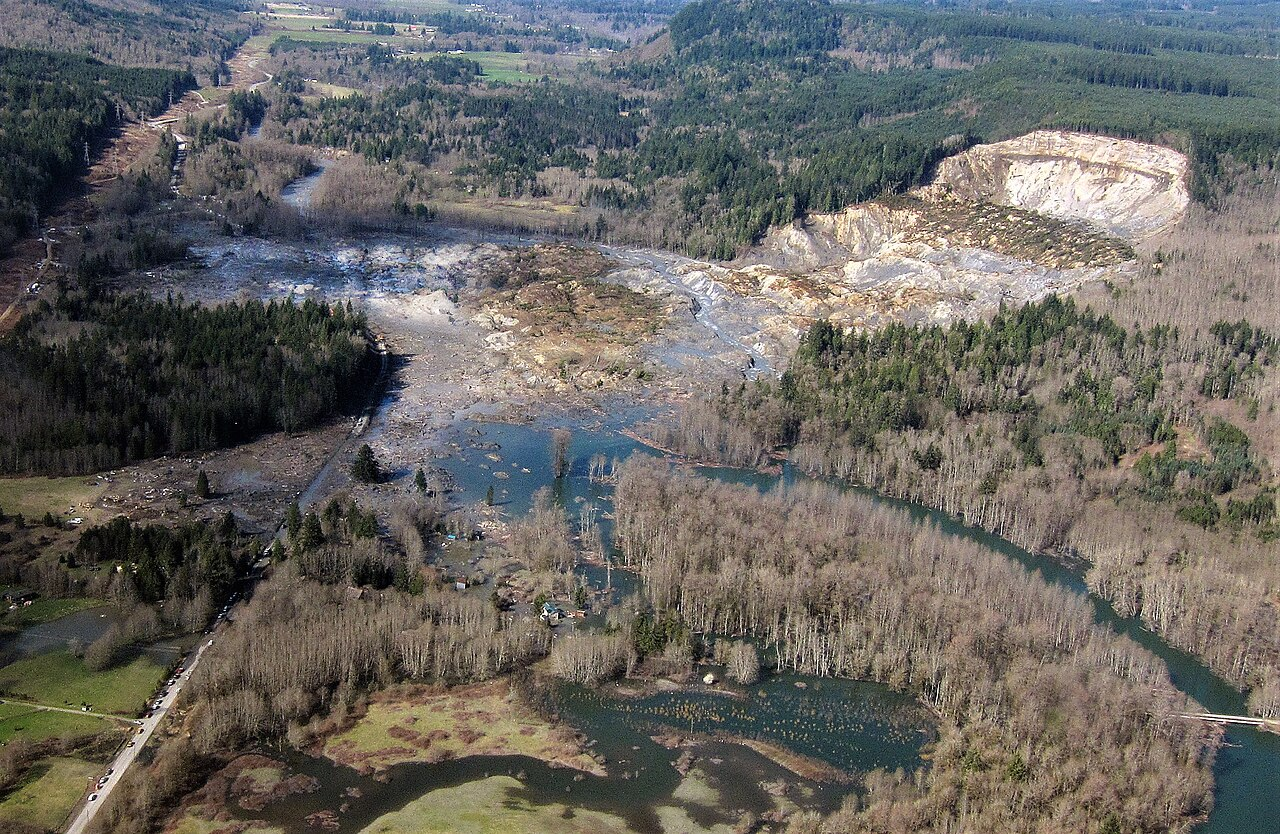
\includegraphics[width=0.6\linewidth]{images/book1/g5-landslide-washington.jpg}

{\small Un grand \omterm{def:g5:natural-hazards:landslide}{glissement de terrain} dans l'État de Washington, aux
États-Unis, en 2014, vu d'avion. Le versant de droite s'est effondré~; sa
\omterm{def:g3:stones-pebbles-sand:sand}{boue} s'est étalée sur toute la \omterm{def:g1:landscapes-around-us:landform}{vallée}, a recouvert une route et a barré la
\omterm{def:g1:landscapes-around-us:water}{rivière}, qui a inondé les bois en amont. Photographie~: Mark Reid, U.S.
Geological Survey (domaine public).}\label{fig:g5:natural-hazards:landslide}
% ledger: usgs:oso-aerial
\end{omfigure}

\section{De l'aléa à la catastrophe}

Une \omterm{def:g5:natural-hazards:storm}{tempête} en plein \omterm{def:g2:water-on-earth:ocean}{océan}, un \omterm{def:g4:volcanoes-earthquakes-first-look:earthquake}{séisme} dans un \omterm{def:g5:weather-and-climate:desert}{désert} vide, une inondation
dans une \omterm{def:g1:landscapes-around-us:landform}{vallée} où personne ne vit~: ce sont des \omterm{def:g5:natural-hazards:hazard}{aléas naturels}, mais ils
ne font de mal à personne. Les mêmes événements deviennent dangereux quand
ils frappent là où vivent des gens.

\begin{definition}[Catastrophe naturelle]\label{def:g5:natural-hazards:disaster}
Il y a \emph{catastrophe naturelle}\index{catastrophe naturelle} quand un
\omterm{def:g5:natural-hazards:hazard}{aléa naturel} frappe un lieu où vivent des gens et fait de grands dégâts~:
des personnes sont blessées ou tuées, des maisons sont détruites, les
routes, l'eau et l'électricité sont coupées.
\end{definition}

\begin{omfigure}
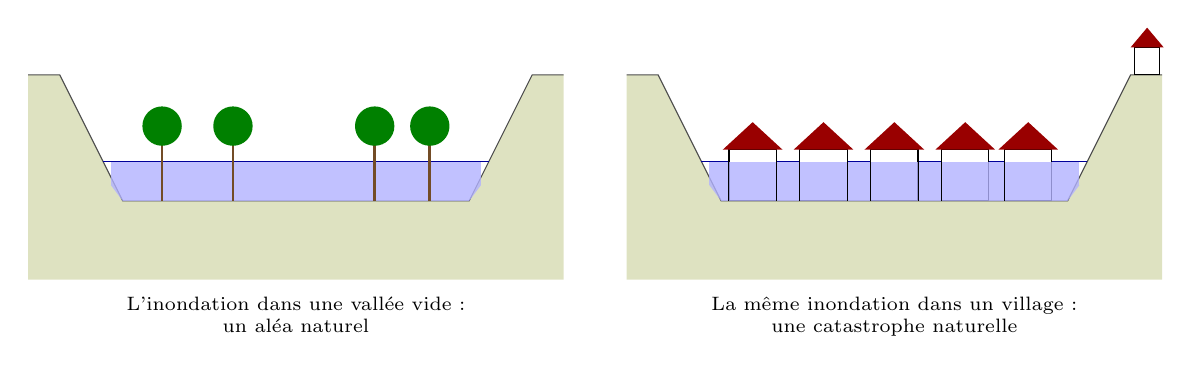
\begin{tikzpicture}[x=1cm, y=1cm, font=\scriptsize]
  \foreach \dx/\title in {0/{L'inondation dans une vallée vide~:\\un aléa naturel},
                          7.6/{La même inondation dans un village~:\\une catastrophe naturelle}} {
    \begin{scope}[xshift=\dx cm]
      % valley sides
      \fill[green!25!brown!30] (0,0) -- (0,2.6) -- (0.4,2.6) -- (1.2,1.0) -- (5.6,1.0)
        -- (6.4,2.6) -- (6.8,2.6) -- (6.8,0) -- cycle;
      \draw[gray!60!black] (0,2.6) -- (0.4,2.6) -- (1.2,1.0) -- (5.6,1.0) -- (6.4,2.6) -- (6.8,2.6);
      % flood water over the whole valley floor
      \fill[blue!30, opacity=0.8] (1.05,1.2) -- (5.75,1.2) -- (5.6,1.0) -- (1.2,1.0) -- cycle;
      \fill[blue!30, opacity=0.8] (1.05,1.2) rectangle (5.75,1.5);
      \draw[blue!60!black] (0.95,1.5) -- (5.85,1.5);
      \node[align=center, anchor=north] at (3.4,-0.1) {\title};
    \end{scope}
  }
  % trees in the empty valley
  \foreach \x in {1.7,2.6,4.4,5.1} {
    \draw[brown!60!black, line width=1pt] (\x,1.0) -- (\x,1.75);
    \fill[green!50!black] (\x,1.95) circle (0.25);
  }
  % houses in the village valley
  \begin{scope}[xshift=7.6cm]
    \foreach \x in {1.6,2.5,3.4,4.3,5.1} {
      \fill[white, draw=black] (\x-0.3,1.0) rectangle (\x+0.3,1.65);
      \fill[red!60!black] (\x-0.38,1.65) -- (\x,2.0) -- (\x+0.38,1.65) -- cycle;
      \fill[blue!30, opacity=0.8] (\x-0.3,1.0) rectangle (\x+0.3,1.5);
    }
    % one house on the high ground, dry
    \fill[white, draw=black] (6.45,2.6) rectangle (6.77,2.95);
    \fill[red!60!black] (6.40,2.95) -- (6.61,3.2) -- (6.82,2.95) -- cycle;
  \end{scope}
\end{tikzpicture}

{\small Deux fois la même inondation. Dans la \omterm{def:g1:landscapes-around-us:landform}{vallée} vide, elle ne fait de
mal à personne~; là où un village a été construit sur la \omterm{def:g5:water-shapes-the-land:flood}{plaine
d'inondation}, elle remplit les maisons. La maison bâtie sur la hauteur
reste au sec.}
\end{omfigure}

Nous ne pouvons pas arrêter une \omterm{def:g5:natural-hazards:storm}{tempête} ou un \omterm{def:g4:volcanoes-earthquakes-first-look:earthquake}{séisme}. Mais nous pouvons
faire beaucoup pour empêcher un aléa de devenir une catastrophe~: construire
loin des \omterm{def:g5:water-shapes-the-land:flood}{plaines d'inondation} et du pied des pentes instables, bâtir des
édifices solides, surveiller le temps et le sol, prévenir les gens à temps,
et apprendre à chacun ce qu'il faut faire.

\subsection*{Les alertes}

Les services \omterm{def:g1:watching-the-weather:weather}{météorologiques} surveillent le ciel jour et nuit. Quand une
\omterm{def:g5:natural-hazards:storm}{tempête}, une canicule ou une inondation approche, ils diffusent des alertes
par la radio, la télévision, le téléphone et internet. Beaucoup de pays
utilisent des couleurs, de la plus calme à la plus grave.

\begin{omfigure}
\begin{tikzpicture}[font=\small, wstep/.style={draw=black!60, minimum width=2.6cm,
    minimum height=0.8cm, font=\small\bfseries, rounded corners=2pt}]
  \node[wstep, fill=green!45] (g) at (0,0) {vert};
  \node[wstep, fill=yellow!60] (y) at (0.6,0.95) {jaune};
  \node[wstep, fill=orange!70] (o) at (1.2,1.9) {orange};
  \node[wstep, fill=red!65, text=white] (r) at (1.8,2.85) {rouge};
  \node[anchor=west] at ($(g.east)+(0.3,0)$) {pas de danger particulier};
  \node[anchor=west] at ($(y.east)+(0.3,0)$) {sois attentif, tiens-toi informé};
  \node[anchor=west] at ($(o.east)+(0.3,0)$) {sois prêt~: un danger est probable};
  \node[anchor=west] at ($(r.east)+(0.3,0)$) {grand danger~: agis tout de suite, suis les consignes};
\end{tikzpicture}

{\small Une échelle de couleurs d'alerte. Le sens exact de chaque couleur
change d'un pays à l'autre~: écoute toujours les consignes données avec
l'alerte.}
\end{omfigure}

\begin{safety}
\textbf{Pendant une \omterm{def:g5:natural-hazards:storm}{tempête}.} Reste à l'intérieur, loin des fenêtres. Ne
sors pas pour regarder, et tiens-toi loin des arbres, qui peuvent tomber,
et des fils électriques tombés au sol.

\textbf{Pendant une inondation.} Monte sur une hauteur ou à un étage
supérieur. Ne traverse jamais l'eau d'une inondation, ni à pied, ni à vélo,
ni en voiture~: un peu d'eau rapide suffit à te faire tomber ou à emporter
une voiture.

\textbf{Pendant une canicule.} Bois de l'eau souvent, reste à l'ombre ou
dans une pièce fraîche aux heures les plus chaudes, et prends des nouvelles
des voisins âgés.

\textbf{Pendant un \omterm{def:g4:volcanoes-earthquakes-first-look:earthquake}{séisme}.} Baisse-toi, abrite-toi, agrippe-toi
(\cref{ch:g4:volcanoes-earthquakes-first-look}).

\textbf{Toujours.} Écoute les alertes et fais tout de suite ce que disent
les personnes responsables.
\end{safety}

\section{Exercices}

\begin{exercise}[$\star$]\label{exo:g5:natural-hazards:1}
Simple \omterm{def:g5:natural-hazards:hazard}{aléa naturel}, ou \omterm{def:g5:natural-hazards:disaster}{catastrophe naturelle}~?
\begin{enumerate}
  \item[(a)] Un \omterm{def:g4:volcanoes-earthquakes-first-look:earthquake}{séisme} secoue un \omterm{def:g5:weather-and-climate:desert}{désert} vide.
  \item[(b)] Une \omterm{def:g5:natural-hazards:storm}{tempête} arrache le toit de nombreuses maisons d'une ville.
  \item[(c)] Un \omterm{def:g5:natural-hazards:landslide}{glissement de terrain} tombe dans une \omterm{def:g1:landscapes-around-us:landform}{vallée} de \omterm{def:g1:landscapes-around-us:landform}{montagne} où personne ne vit.
  \item[(d)] Une \omterm{def:g1:landscapes-around-us:water}{rivière} inonde un village et remplit ses maisons d'eau.
\end{enumerate}
\end{exercise}

\begin{exercise}[$\star$]\label{exo:g5:natural-hazards:2}
Classe ces aléas en trois familles (venus de l'air, venus de l'eau, venus
du sol)~: un \omterm{def:g5:natural-hazards:landslide}{glissement de terrain}~; une canicule~; une inondation~; une
\omterm{def:g4:volcanoes-earthquakes-first-look:eruption}{éruption} volcanique~; une \omterm{def:g5:natural-hazards:storm}{tempête}~; une \omterm{def:g5:natural-hazards:drought}{sécheresse}~; un \omterm{def:g4:volcanoes-earthquakes-first-look:earthquake}{séisme}.
\end{exercise}

\begin{exercise}[$\star$]\label{exo:g5:natural-hazards:3}
Qu'est-ce qu'une \omterm{def:g5:natural-hazards:drought}{sécheresse}~? Donne deux façons dont une longue \omterm{def:g5:natural-hazards:drought}{sécheresse} nuit aux gens.
\end{exercise}

\begin{exercise}[$\star$]\label{exo:g5:natural-hazards:4}
La radio annonce une alerte rouge à la \omterm{def:g5:natural-hazards:storm}{tempête} pour cette nuit. Donne trois
choses que ta famille devrait faire.
\end{exercise}

\begin{exercise}[$\star$]\label{exo:g5:natural-hazards:5}
Une grande \omterm{def:g5:natural-hazards:storm}{tempête} tournante, avec un œil, se forme au-dessus d'une \omterm{def:g2:water-on-earth:ocean}{mer}
tropicale chaude. Comment l'appelle-t-on si elle frappe (a) la \omterm{def:g1:landscapes-around-us:water}{côte} de la
Floride, dans l'Atlantique Nord~; (b) le Japon, dans le Pacifique
Nord-Ouest~; (c) la \omterm{def:g1:landscapes-around-us:water}{côte} de l'Inde, sur l'\omterm{def:g2:water-on-earth:ocean}{océan} Indien~?
\end{exercise}

\begin{exercise}[$\star$]\label{exo:g5:natural-hazards:6}
Range les quatre couleurs d'alerte dans l'ordre, de la plus calme à la plus
grave. Que dois-tu faire au niveau le plus grave~?
\end{exercise}

\begin{exercise}[$\star\star$]\label{exo:g5:natural-hazards:7}
Regarde la photographie du \omterm{def:g5:natural-hazards:landslide}{glissement de terrain},
page~\pageref{fig:g5:natural-hazards:landslide}. Décris ce que le
\omterm{def:g5:natural-hazards:landslide}{glissement de terrain} a fait à la \omterm{def:g1:landscapes-around-us:landform}{vallée}~: au versant, à la route et à la
\omterm{def:g1:landscapes-around-us:water}{rivière}. Pourquoi les terres situées en amont sont-elles maintenant sous
l'eau~?
\end{exercise}

\begin{exercise}[$\star\star$]\label{exo:g5:natural-hazards:8}
Tom dit~: «~Les inondations sont naturelles, donc on ne peut rien y
faire.~» Lena dit~: «~Nous ne pouvons pas empêcher une \omterm{def:g1:landscapes-around-us:water}{rivière} de déborder,
mais nous pouvons empêcher une inondation de devenir une catastrophe.~»
Qui a raison~? Explique avec deux exemples.
\end{exercise}

\begin{exercise}[$\star\star$]\label{exo:g5:natural-hazards:9}
Dans une région agricole imaginaire, il tombe habituellement environ
60 millimètres de \omterm{def:g4:clouds-rain-snow:precipitation}{pluie} chaque mois. Pendant une \omterm{def:g5:natural-hazards:drought}{sécheresse}, il n'est
tombé, chacun des quatre mois, que le quart de la \omterm{def:g4:clouds-rain-snow:precipitation}{pluie} habituelle.
\begin{enumerate}
  \item[(a)] Combien de \omterm{def:g4:clouds-rain-snow:precipitation}{pluie} tombe-t-il habituellement en quatre mois~?
  \item[(b)] Combien en est-il tombé pendant la \omterm{def:g5:natural-hazards:drought}{sécheresse}, en quatre mois~?
  \item[(c)] Combien de \omterm{def:g4:clouds-rain-snow:precipitation}{pluie} a manqué~?
\end{enumerate}
\end{exercise}

\begin{exercise}[$\star\star$]\label{exo:g5:natural-hazards:10}
Une ville imaginaire compte 1\,200 logements. Un quart d'entre eux se
trouvent dans la \omterm{def:g5:water-shapes-the-land:flood}{plaine d'inondation} de sa \omterm{def:g1:landscapes-around-us:water}{rivière}.
\begin{enumerate}
  \item[(a)] Combien de logements se trouvent dans la \omterm{def:g5:water-shapes-the-land:flood}{plaine d'inondation}~?
  \item[(b)] La ville aide les propriétaires d'un tiers de ces logements à
        s'installer sur une hauteur. Combien de logements restent dans la \omterm{def:g5:water-shapes-the-land:flood}{plaine d'inondation}~?
\end{enumerate}
\end{exercise}

\begin{exercise}[$\star\star\star$]\label{exo:g5:natural-hazards:11}
Deux villages éloignés l'un de l'autre sont frappés la même nuit par des
\omterm{def:g5:natural-hazards:storm}{tempêtes} de même force. Dans le premier, personne n'est blessé et les
dégâts sont faibles. Dans le second, beaucoup de maisons sont détruites.
Donne au moins trois raisons différentes qui pourraient expliquer cette
différence.
\end{exercise}
